%
%----------------------------------------------------------------------------------------
%	PACKAGES AND DOCUMENT CONFIGURATIONS
%----------------------------------------------------------------------------------------
%

\documentclass[12pt]{article} %report, article, amsart, exam
\usepackage[letterpaper,margin=1in]{geometry}
\usepackage{fancyhdr,color}
\usepackage{tikz,graphicx,multicol}
\usepackage{amssymb,euscript,eufrak,nicefrac,enumitem}
\usepackage{amsfonts,amsmath,amsthm} %don't need with 'amsart' document class
\usepackage{hyperref}
\usepackage{comment}
\usepackage{scrextend} %needed for addmargin environment
\usepackage{graphicx} 
\usepackage{listings}
\usepackage{color}
\usepackage{accsupp}
\usepackage{booktabs}
\usepackage{subcaption}

\definecolor{dkblue}{rgb}{0,0,0.5}
\definecolor{comment}{rgb}{1,0,0}
\definecolor{mauve}{rgb}{.627,.126,.941}
\definecolor{purple}{rgb}{0.5, 0, 0.545098}

%
%----------------------------------------------------------------------------------------
%% Define headers & footers
%----------------------------------------------------------------------------------------

\pagestyle{fancy}
   \lhead{} 
   %\chead{Loyola University Chicago} 
   \rhead{}
   \renewcommand{\headrulewidth}{0pt}
   \addtolength{\footnotesep}{5mm}
 
%
%----------------------------------------------------------------------------------------
%% Some user-defined colors
%----------------------------------------------------------------

\setlength{\parskip}{1em}
\renewcommand{\baselinestretch}{1.3}

%
%----------------------------------------------------------------------------------------
%% BEGIN: topmatter
%----------------------------------------------------------------------------------------
%

\title{ COMP 464 - High Performance Computing \\ OpenMP Threading} % Title
\author{
Loyola University Chicago \\
Jose Luis Rodriguez 
} % Author name
\date{\today} % Date for the report

%
%% END: topmatter
%%------------------------------

\begin{document}

\maketitle

\thispagestyle{fancy}

%---------------------------------------------------------------------------------------- 
%	SECTION 1 - PROBLEM STATEMENT
%----------------------------------------------------------------------------------------

\section{Overview}

This report highlights the procedures and results of running the nbody3 C++ code that predicts the individual motion of a group of celestial objects (particles) interacting with each other gravitationally. The program also runs a series of experiments and generates a benchmark (max, min and average speed) utilizing the Stampede2 supercomputer at The University of Texas at Austin's Texas Advanced Computing Center (TACC). The nbody3 code utilize Intel C++ library compilers and the OpenMP library in order to parallelize the serial code details and specifications to follow. 

The n-body problem code performs two major benchmarks, strong scalability and weak scalability. 
Run serial and parallel cases with 1,000, 2,000, 4,000, and 8,000 particles using 1, 2, 4, 8, 16, 32, and 64 threads. (Stampede2 KNL nodes have 68 cores and each core can run 4 hardware threads so you can try with more threads if you like.) Record the average time per step. Make sure you use enough steps to give consistent results. These results will be used to compute the strong scalability and efficiency.

Now run a weak scalability test. The goal here is to keep the workload per-thread constant. This means you need to increase the number of particles when you increase the number of threads. Start with 200 and 1,000 particles serially and determine how many particles are needed when you double the number of threads and continue this up to 64 threads. Recall that the n-body problem cost scales as n2 where n is the \# of particles. Use that to determine how to increase the \# of particles per thread.

The n-body problem benchmark runs a number of tests measuring the bandwidth of L1, L2, L3 cache, and main DRAM. The first benchmark uses GNU C++ compiler to build the Stream2 program on Stampede2 compute and login nodes as well as and the Lenovo workstation. After building the code with GNU or Intel compiler, the program is run and the output is recorded in the tables below. The specifications of each system are also recorded in the tables at the end of the report. The idea behind this experiment is to examine how the memory and cache behave during the different experience and to compare the Intel and GNU C++ compilers. 

%----------------------------------------------------------------------------------------
%	SECTION 2 - DESCRIPTION
%----------------------------------------------------------------------------------------

% Report a brief report that summarizes the performance results you measured.
% Create plots strong scaling speed-up and efficiency ( Lecture #1 ) 
% Create plots weak scaling efficiency.
%
% Use these plots to answer:
% (1) does the n-body algorithm scale in parallel 
% (2) is the scalability constant or dependent upon the number of threads and particles?
%
% Also include a summary of code modifications that were necessary.

\section{Benchmark Analysis}

%  strong scalability 

% weak scalability

The stream2 code runs a number of loops over a sequence of experiments and various benchmarks:

\begin{table}[ht]
\centering
\resizebox{\textwidth}{!}{%
\begin{tabular}{cl}
\textbf{Benchmark} & \textbf{Description} \\ \midrule
FILL (MB/s) & Set all elements in an array to a particular value \\
COPY & Copy two arrays - one into the other \\
AXPY & Takes two arrays make changes and writes back (Alpha x plus y) \\
DOT & Sum of the product of two arrays (Dot Product) \\ \bottomrule
\end{tabular}%
}
\end{table}

The benchmarks above were run on Stampede2 following two approaches. The first the code runs on the compute Node by requesting a flat quadrant and executing the code on that node. The second approach uses the $numactl$ command to run the code using the MCDRAM on the computer node. 

The benchmarks were run with a min array size of 30 Bytes and three different max array sizes (20Mb, 25Mb, and 30Mb).This report only highlights the results when using the largest array size (30Mb) as the goal is to stress the last level cache and setting the number of tests between the min and max array size to 50. The same parameters were used for all benchmarks, compilers and nodes. To calculate the size of the array at the $n$ iteration the following metric was used:

\begin{table}[ht]
\resizebox{\textwidth}{!}{%
\begin{tabular}{cc}
\textbf{Benchmark} & \textbf{Array Size (Metric) } \\  \midrule
FILL  & $(\text{n\_iteration})(8 \text{ bytes/double})(1 \text{ double/iteration})$ \\
COPY & $(\text{n\_iteration})(8 \text{ bytes/double})(2 \text{ double/iteration})$ \\
AXPY & $(\text{n\_iteration})(8 \text{ bytes/double})(3 \text{ double/iteration})$ \\
DOT & $(\text{n\_iteration})(8 \text{ bytes/double})(2 \text{ double/iteration})$ \\ \bottomrule
\end{tabular}%
}
\end{table}

\newpage

\subsection{Benchmark Results}

In Figure.1 Stampede2 compute node using the GNU compiler, we can see how the benchmark that uses most bandwidth is the \textsc{COPY} benchmark, with a top performance at $26kb$ right before filling the $32kb$ L1 cache then we see another drop at approximately after 534kb array size when L2 cache gets  filled. The other benchmarks seem to behave more or less similarly, some of them show some drops but nothing close to what the \textsc{COPY} benchmark experience.

\begin{figure}[htb]
\caption{Stampede2 Compute Node - GNU Compiler}\label{fig:benchmark01}
\centering
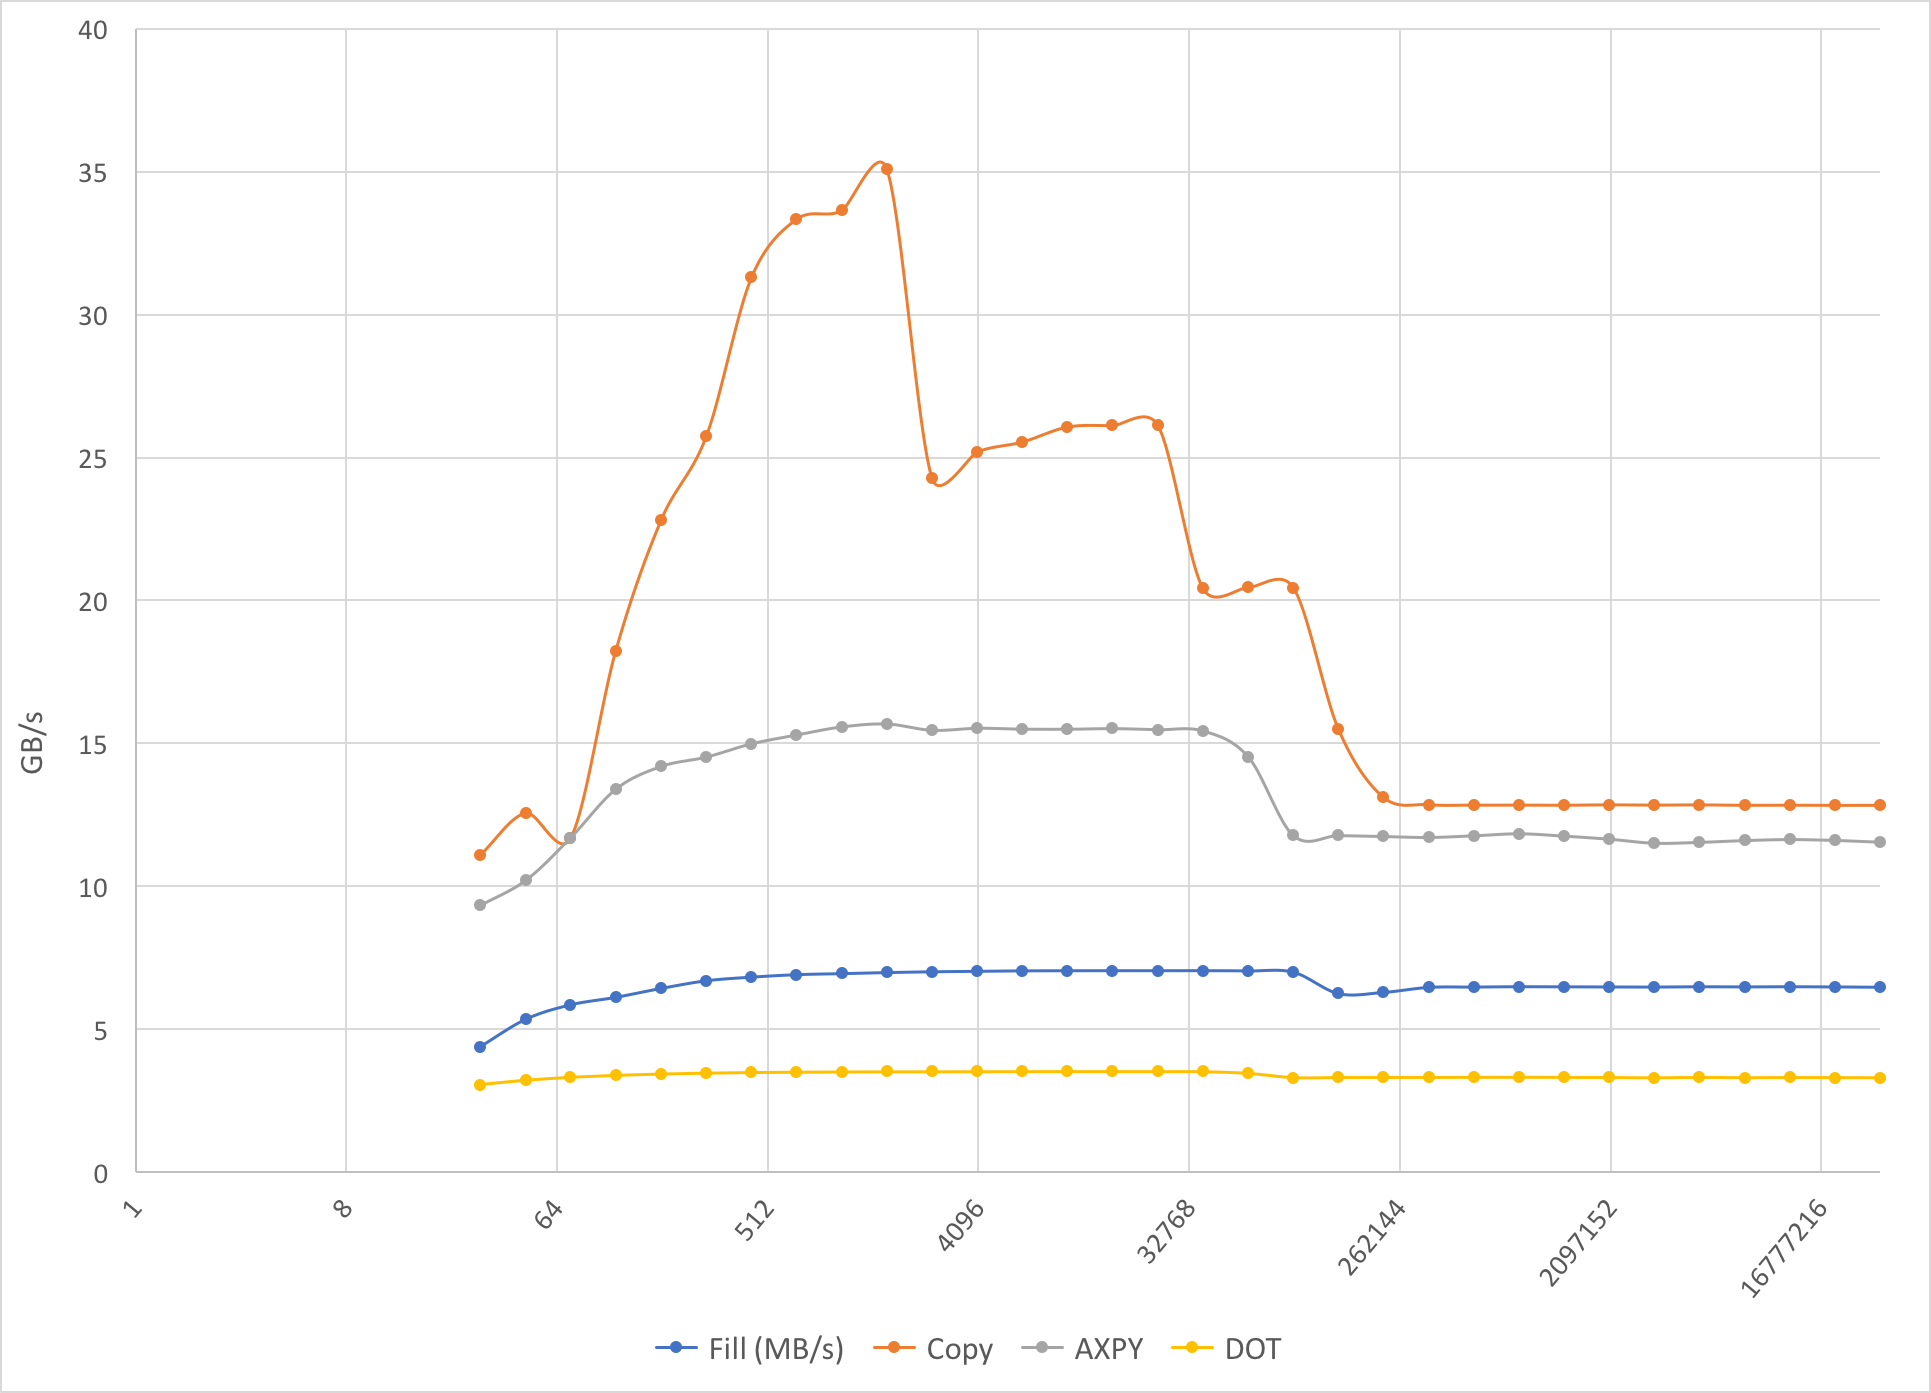
\includegraphics[width=\textwidth,keepaspectratio]{imgs/img01.png}
\end{figure} 

\newpage

Now in Figure.2 we change the compiler to Intel's C++ compiler and we can see significant changes on all the benchmarks. The most prominent change from the previous figure is the \textsc{AXPY}  benchmark that peeks approximately around $40kb$ with a much higher bandwidth almost 120 times higher compared with the GNU compiler.  The \textsc{FILL} benchmark also shows signs of a significant drop with a peek at 32kb and $100$Gb\/s to $40$Gb\/s  after the $L1$ gets filled.

\begin{figure}[htb]
\caption{Stampede2 Compute Node - Intel Compiler}\label{fig:benchmark02}
\centering
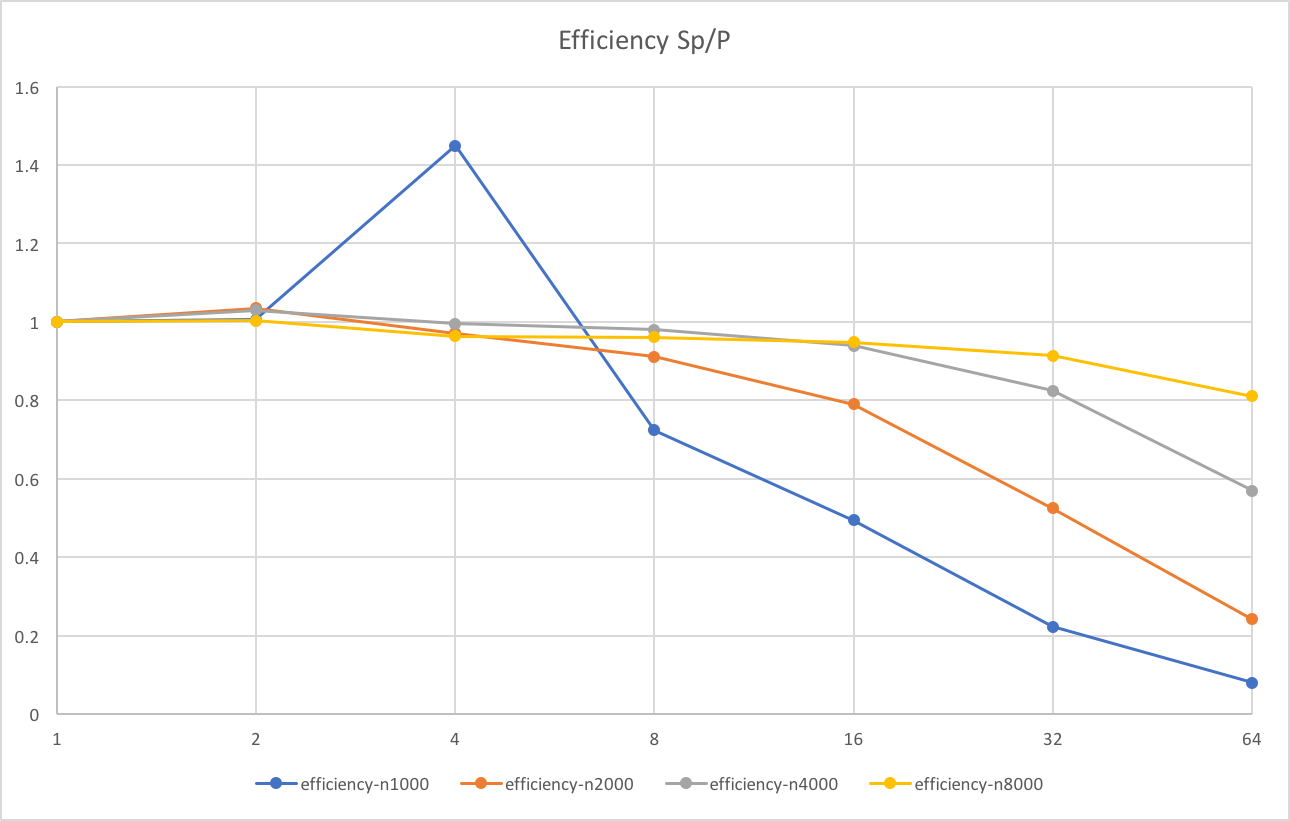
\includegraphics[width=\textwidth,keepaspectratio]{imgs/img02.png}
\end{figure}

\newpage

%----------------------------------------------------------------
%	SECTION 3 - REFERENCE
%----------------------------------------------------------------

\section{Reference}

\begin{flushleft}
Stampede2 User Guide -- Managing Memory \\ \url{https://portal.tacc.utexas.edu/user-guides/stampede2#managingmemory}

Introduction to High Performance Scientific Computing -- Victor Eijkhout \\ \url{http://pages.tacc.utexas.edu/~eijkhout/istc/istc.html}
\end{flushleft}

\begin{table}[]
\centering
\caption{Stampede2 - Compute Node (knl) - System Information}
\resizebox{\textwidth}{!}{%
\begin{tabular}{@{}ll@{}}
\toprule
\textbf{Architecture} & x86\_64 \\ \midrule
\textbf{CPU op-mode(s)} & 32-bit, 64-bit \\
\textbf{Byte Order} & Little Endian \\
\textbf{CPU(s)} & 272 \\
\textbf{On-line CPU(s) list} & 0-271 \\
\textbf{Thread(s) per core} & 4 \\
\textbf{Core(s) per socket} & 68 \\
\textbf{Socket(s)} & 1 \\
\textbf{NUMA node(s)} & 2 \\
\textbf{Vendor ID} & GenuineIntel \\
\textbf{CPU family} & 6 \\
\textbf{Model} & 87 \\
\textbf{Model name} & Intel(R) Xeon Phi(TM) CPU 7250 @ 1.40GHz \\
\textbf{Stepping} & 1 \\
\textbf{CPU MHz} & 1255.132 \\
\textbf{BogoMIPS} & 2793.44 \\
\textbf{L1d cache} & 32K \\
\textbf{L1i cache} & 32K \\
\textbf{L2 cache} & 1024K \\
\textbf{NUMA node0 CPU(s)} & 0-271 \\
\textbf{NUMA node1 CPU(s)} &  \\ \bottomrule
\end{tabular}%
}
\end{table}

\begin{table}[]
\centering
\caption{Stampede2 Compute Node - GNU Compiler}
\resizebox{\textwidth}{!}{%
\begin{tabular}{@{}llllll@{}}
\toprule
\textbf{Size (iterations)} & \textbf{Fill (MB/s)} & \textbf{Copy} & \textbf{AXPY} & \textbf{DOT} & \textbf{Uncertainty (\%)} \\ \midrule
30 & 4393.162231 & 11104.6881 & 9336.596419 & 3051.421911 & 1.90\% \\
47 & 5350.378441 & 12565.39118 & 10220.65398 & 3209.223289 & 1.50\% \\
73 & 5853.695055 & 11687.71559 & 11702.86902 & 3316.590107 & 1.10\% \\
114 & 6116.984412 & 18242.91233 & 13398.08149 & 3388.55338 & 0.70\% \\
178 & 6427.522021 & 22800.19441 & 14194.47704 & 3438.065904 & 0.50\% \\
279 & 6698.122428 & 25768.72093 & 14527.06717 & 3472.020319 & 0.30\% \\
435 & 6824.597812 & 31305.48923 & 14986.95631 & 3493.9909 & 0.20\% \\
679 & 6911.333146 & 33345.25901 & 15297.0655 & 3507.619116 & 0.10\% \\
1060 & 6948.028771 & 33650.79479 & 15578.51236 & 3515.477478 & 0.10\% \\
1656 & 6985.001187 & 35089.74094 & 15680.55274 & 3520.668913 & 0.10\% \\
2586 & 7012.81148 & 24271.79651 & 15462.08087 & 3521.383827 & 0.00\% \\
4038 & 7029.597848 & 25202.06851 & 15531.84052 & 3525.104143 & 0.00\% \\
6305 & 7044.938436 & 25549.57693 & 15502.22589 & 3527.599249 & 0.00\% \\
9846 & 7050.075265 & 26072.88131 & 15498.96218 & 3529.112917 & 0.00\% \\
15374 & 7051.78082 & 26124.29129 & 15519.55808 & 3528.904854 & 0.00\% \\
24008 & 7050.994641 & 26121.05296 & 15482.61471 & 3527.958451 & 0.00\% \\
37488 & 7051.782966 & 20421.04818 & 15437.97559 & 3523.761178 & 0.00\% \\
58539 & 7042.233872 & 20459.72158 & 14530.19158 & 3463.650355 & 0.00\% \\
91410 & 6996.433371 & 20445.17519 & 11782.12811 & 3306.784882 & 0.00\% \\
142738 & 6248.110944 & 15491.29423 & 11778.74414 & 3309.431658 & 0.00\% \\
222889 & 6290.558991 & 13109.06205 & 11746.50454 & 3311.366333 & 0.00\% \\
348047 & 6464.796754 & 12858.42716 & 11715.18304 & 3313.983805 & 0.00\% \\
543483 & 6477.457041 & 12841.93352 & 11772.74996 & 3316.270979 & 0.00\% \\
848661 & 6489.448093 & 12842.14791 & 11843.17557 & 3319.445295 & 0.00\% \\
1325203 & 6485.506785 & 12838.69628 & 11761.03164 & 3314.821514 & 0.00\% \\
2069336 & 6480.942411 & 12851.09811 & 11653.18953 & 3309.260037 & 0.00\% \\
3231315 & 6477.659875 & 12842.6458 & 11513.15796 & 3300.587295 & 0.00\% \\
5045773 & 6487.756168 & 12849.37284 & 11543.48494 & 3313.220334 & 0.00\% \\
7879091 & 6483.470428 & 12836.38542 & 11605.7627 & 3304.53413 & 0.00\% \\
12303381 & 6488.676065 & 12838.86536 & 11641.5715 & 3308.75048 & 0.00\% \\
19212013 & 6481.651785 & 12834.44793 & 11610.01186 & 3306.78088 & 0.00\% \\
30000000 & 6470.497548 & 12835.64937 & 11548.34264 & 3302.602269 & 0.00\% \\ \bottomrule
\end{tabular}%
}
\end{table}

\end{document}